\documentclass{article}
\usepackage{graphicx} % Required for inserting images
\usepackage{geometry}
\usepackage{pgfplots}
<<<<<<< HEAD
	\pgfplotsset{width=8cm, compat=1.9}
	\usepackage{tikz}
	% We will externalize the figures
	\usepgfplotslibrary{external}
	\tikzexternalize
	\usepgfplotslibrary{fillbetween}
	
\usepackage{multicol}
=======
\usepackage{float}
>>>>>>> a3d9df66a0422b892d6552d2fbb6390c4b8811f8

\title{Mathematik - Zusammenfassung fürs Abitur}
\author{Maximilian Penke}
\date{January 2024}
\newgeometry{vmargin={15mm}, hmargin={12mm,17mm}}

\renewcommand*\contentsname{Gliederung}

\begin{document}

\maketitle

\begin{abstract}
    Dies ist eine Zusammenfassung für die Inhalte des Berliner Abiturs von 2024 im Fach Mathematik. Dabei ist des in die drei Hauptthemen unterteilt, wobei es jeweils Differenzierungen gibt. Dafür werden die Inhalte der Einzelthemen erklärt, mit der allgemeinen Umsetzungsweise versehen und darauf folgend mit unterschiedlichen Beispielen.
\end{abstract}

\tableofcontents
\newpage

\section{Analysis}
	\subsection{Gleichungen und Gleichungssysteme}
		\paragraph{Gleichung}
			Eine Gleichung beschreibt das Verhältnis von zwei Termen mit einem sog. Gleichungsoperator ($=$,$<$,$>$,$<=$,$>=$,$\neq$).
			Eine Gleichung kann nur aus Zahlen bestehen (1=1; $1<2$; $4\neq5$; usw.),
			aber auch aus Variablen (a=b; x=5; $z^2=25$).
		\paragraph{Gleichungssysteme}\label{Gleichungssysteme}
			Eine Reihe von Gleichungen, die im selben Kontext stimmen, nennt man Gleichungssystem. Die Gleichungen eines Gleichungssystems werden meist
			mit römischen Ziffern (I; II; III) denotiert. Beispiel:
			\[ I \quad 5a+2b+c=0\]
			\[ II \quad -2a+b=5\]
			\[ III \quad c-10=0\]

<<<<<<< HEAD
			Mit einem solchen Gleichungssystem sind wir in der Lage, die Werte der Variablen herauszufinden.  An unserem Beispiel würde das wie folgt aussehen:
			
			\[ III \quad c-10=0 \quad | +10 \]
			\[c = 10\]
			c=10 in I einsetzen: 
			\[ I \quad 5a+2b+10=0 \quad | -2b \quad -10\]
			\[ 5a=-2b-10 \quad | \div 5\]
			\[a=-\frac{2}{5}b-10\]
			$a=-\frac{2}{5}b-10$ in II einsetzen:
			\[ II \quad -2(-\frac{2}{5}b-10)+b=5\]
			\[ \frac{4}{5}b+20=5 \quad | -20\]
			\[ \frac{4}{5}b=-15 \quad |\cdot \frac{5}{4} \]
			\[ b=-18.75\]
			b=-18.75 und c=10 in I einsetzen:
			\[ I \quad 5a+2(-18.75)+10=0 \quad | -10 \]
			\[ 5a-37.5=-10 \quad |+37.5 \]
			\[ 5a = 27.5 \quad | \div 5\]
			\[ a = 5.5\]
			
			Also ist $a=5.5$, $b=-18.75$, $c=10$
			
			Gleichungsysteme können auch zur Rekonstruktion von Funktionen verwendet werden (siehe \ref{Rekonstruktion}). 
=======
Mit einem solchen Gleichungssystem sind wir in der Lage, die Werte der Variablen herauszufinden. An unserem Beispiel würde das wie folgt aussehen:
>>>>>>> a3d9df66a0422b892d6552d2fbb6390c4b8811f8

	\subsection{Differenzialrechnung}
		\paragraph{Was ist Differenzialrechnung?}
			Um lokale Änderungen/Steigungen von Funktionen zu bestimmen kann man die Differenzialrechnung verwenden.
			Man kann mit ihr ebenfalls Steigungsänderungen bestimmen.
		\paragraph{Steigerungsbestimmung von Funktionen über Intervalle}

<<<<<<< HEAD
			Um die Steigung von Funktionen über Intervalle zu betrachten sind typische Steigungsdreiecke praktisch,
			da man sie visuell gut darstellen kann und sie ein Werkzeug sind welches in der Mittelstuffe bereits
			Verwendung gefunden hat.
			 
			Differenzenquotient:
			\[
			    m = {\frac {\Delta y} {\Delta x}}
			\]
			
			Differenzialquotient:
			\[
			    m = \lim_{x \to x_{0}} {{f(x_{0}) - f(x)} \over { x_{0} - x}}
			\]
=======
Also ist $a=5.5$, $b=-18.75$, $c=10$

Gleichungsysteme können auch zur Rekonstruktion von Funktionen verwendet werden (siehe \ref{Rekonstruktion}). 

\subsection{Funktionen}
Eine mathematische Funktion $f$ ordnet jedem Wert $x$ in ihrem Definitionsbereich (siehe \ref{Definitionsbereich})
einen Wert $y$ zu. Sie wird denotiert mit der Formulierung $y=f(x)= $ die Definition der Funktion (z.B. $x^2-5x+6$).
Der Graph einer Funktion ist die visuelle Abbildung der Funktion. In der Schule kennen wir 5 Arten von Funktionen:
\begin{enumerate}
    \item Polynomfunktionen ($ax+bx^2+cx^3+...+nx^m$)
    \item Wurzelfunktionen ($ \sqrt[3]{x} $ mit $ (\sqrt[3]{x})^3=x $. Statt x kann auch eine Funktion im Radikant stehen.)
    \item Exponentialfunktionen ($a^{x}$, häufiger $n \cdot e^x$, e ist die sog. \emph{Eulersche Zahl}. Statt x kann auch eine Funktion im Exponent stehen.)
    \item Logarithmusfunktionen ($log_2(x)$, häufiger $n \cdot ln(x)$, mit $e^{ln(x)}=x$. Statt x kann auch eine Funktion im Radikant stehen.)
    \item Gebrochenrationale Funktionen ($\frac{1}{g(x)}$, $g(x)$ kann jede beliebige Funktion sein.)

\end{enumerate}

\subsubsection{Spezielle Punkte}\label{Spezielle Punkte}

Generell gilt: immer den x-Wert herausfinden, wenn gefordert den y-Wert herausfinden. Dazu x in f(x) einsetzen.

\begin{enumerate}
    \item Nullstellen: $f(x)=0$
    \item Y-Achsenabschnitt: $x=0 \rightarrow y=f(0)$
    \item Tiefpunkt: $f'(x)=0$, $f''(x)>0$
    \item Hochpunkt: $f'(x)=0$, $f''(x)<0$
    \item Wendepunkt: $f''(x)=0$, $f'''(x)\neq 0$.
    \item Sattelpunkt: $f'(x)=0$, $f''(x)=0$
\end{enumerate}

\subsection{Funktionsscharen}

Funktionen müssen nicht nur einen Eingabewert haben. Eine Funktion $f$ kann auch von mehreren Werten abhängen.
Das Volumen $V$ eines Quaders beispielsweise, hängt von der Länge, Breite und Tiefe des Quaders ab.
Also ist das Volumen: $V(l,b,t)=l \cdot b \cdot t$. Im Abitur werden solche Funktionen allerdings nicht verwendet.
Stattdessen gibt es \emph{Funktionsscharen}. Diese haben einen zweiten Parameter, der Scharparameter genannt wird.
Eine Funktionsschar wird wie folgt geschrieben: $y=f_a(x)$ mit a als Scharparameter. Setzt man für a einen Wert ein,
so erhält man eine Scharfunktion der Funktionsschar. Eine Scharfunktion mit $a=2$: $y=f_2(x)$.

\subsubsection{Bestimmung des Parameter mit gegebenem x und y}
Häufig sind x, y und die Funktion gegeben und es gilt den Scharparameter herauszufinden. Dazu setzt man jeden bekannten
Wert ein und stellt nach a um. Beispiel: Eine Scharfunktion der Funktionsschar $f_a(x)=2^{x-a}$
verläuft durch den Punkt (5|8). Berechne a.

\[ 8=2^{5-a} \quad | log_2() \]
\[ 3=5-a \quad | +a \quad -3 \]
\[ a=2 \]

\subsubsection{Berechnung typischer Punkte in Abhängigkeit vom Parameter}
Eine Funktionsschar hat meistens Nullstellen, einen Y-Achsenabschnitt und Extrempunkte. Die Position dieser,
hängt von dem Scharparameter ab. Die Berechnung typischer Punkte erfolgt auf die exakt selbe Art und Weise,
wie bei normalen Funktionen (siehe \ref{Spezielle Punkte})

\subsubsection{Ortskurve}

Die Ortskurve ist eine Funktion, auf der alle Extrempunkte der Scharfunktionen einer Funktionsschar liegen. Beispiel:

\begin{figure}[H]
\centering
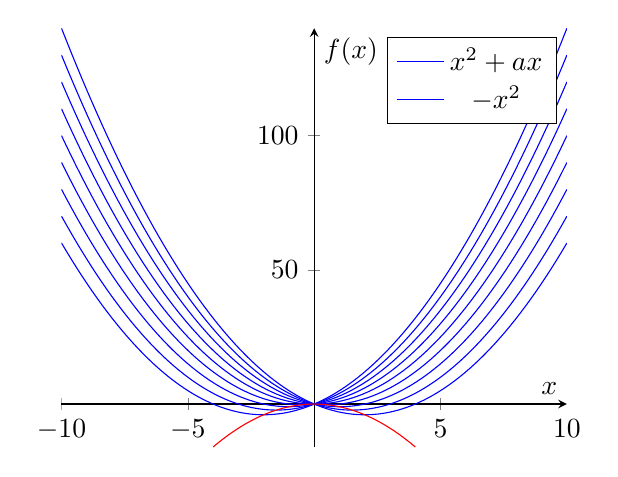
\begin{tikzpicture}
    \begin{axis}[
        axis lines = center,
        xlabel = \(x\),
        ylabel = {\(f(x)\)},
    ]
    %Below the red parabola is defined
    \addplot [
        domain=-10:10, 
        samples=100, 
        color=blue,
    ]
    {x^2 - 2*x};
    %Here the blue parabola is defined
    \addplot [
        domain=-10:10, 
        samples=100, 
        color=blue,
        ]
        {x^2 + 2*x};
    \addplot [
        domain=-10:10, 
        samples=100, 
        color=blue,
    ]
    {x^2 - x};
    %Here the blue parabola is defined
    \addplot [
        domain=-10:10, 
        samples=100, 
        color=blue,
        ]
        {x^2 + x};
    \addplot [
        domain=-10:10, 
        samples=100, 
        color=blue,
    ]
    {x^2 - 3*x};
    %Here the blue parabola is defined
    \addplot [
        domain=-10:10, 
        samples=100, 
        color=blue,
        ]
        {x^2 +3*x};
        \addplot [
            domain=-10:10, 
            samples=100, 
            color=blue,
            ]
            {x^2 + 4*x};
        \addplot [
            domain=-10:10, 
            samples=100, 
            color=blue,
        ]
        {x^2 - 4*x};
        \addplot [
        domain=-10:10, 
        samples=100, 
        color=blue,
        ]
        {x^2};
    \addlegendentry{\(x^2 + ax\)}
    \addplot [
        domain=-4:4, 
        samples=100,
        color=red,
    ]
    {-x^2};
    \addlegendentry{\(-x^2\)}
    
\end{axis}
\end{tikzpicture}
\end{figure}    

\subsubsection{Gemeinsame Punkte}

\subsection{Differenzialrechnung}
\paragraph{Was ist Differenzialrechnung?}

Um lokale Änderungen/Steigungen von Falsunktionen zu bestimmen kann man die Differenzialrechnung verwenden.
Man kann mit ihr ebenfalls Steigungsänderungen bestimmen.
\paragraph{Steigerungsbestimmung von Funktionen über Intervalle}

Um die Steigung von Funktionen über Intervalle zu betrachten sind typische Steigungsdreiecke praktisch,
da man sie visuell gut darstellen kann und sie ein Werkzeug sind welches in der Mittelstuffe bereits
Verwendung gefunden hat.

Differenzenquotient:
\[
    m = {\frac {\Delta y} {\Delta x}}
\]

Differenzialquotient:
\[
    m = \lim_{x \to x_{0}} {{f(x_{0}) - f(x)} \over { x_{0} - x}}
\]
>>>>>>> a3d9df66a0422b892d6552d2fbb6390c4b8811f8



		\paragraph{}

<<<<<<< HEAD
	\subsection{Ableitungsregeln und Ableitungsbegriff}\label{Ableitungen}
	
	\subsection{Integralrechnung}\label{Integralrechnung}
=======
\subsection{Ableitungsregeln und Ableitungsbegriff}\label{Ableitungen}
\subsection{Integralrechnung}\label{Integralrechnung}

\subsection{Grenzwerte}
\subsection{Definitionsbereich und Definitionslücken}\label{Definitionsbereich}
\subsection{Rekonstruktion}\label{Rekonstruktion}
\paragraph{}
Zur Rekonstruktion einer Funktion werden gewisse Bedingungen vorrausgesetzt, die in ein Gleichungssystem (siehe \ref{Gleichungssysteme}) umgewandelt werden können.
Beispiel: Ein Helikopterflug kann annährend durch eine Parabel beschrieben werden (Zeit auf der x-Achse in Minuten, Höhe auf der Y-Achse in Kilometer). \\
Der Helikopter erreicht seine maximale Flughöhe von 10 nach 20 Minuten. ( $ \rightarrow f(20)=10 \rightarrow f'(20)=0 $ ) \\
Der Helikopter hebt bei t=0 ab. ($ \rightarrow f(0)=0$) \\

\[ I \quad 10=400a+20b+c \]
\[ II \quad 0=40a+b \]
\[ III \quad c=0 \]

c=0 in I einsetzen:

\[I \quad 10=400a+20b \quad |-400a \]
\[ 10-400a=20b \quad | \div 20\]
\[ 0.5-20a=b\]

$b= 0.5-20a $ in II einsetzen:

\[ 0=40a+(0.5-20a)\]
\[ 0=20a+0.5 \quad |-0.5 \quad \div 20\]
\[ a=-\frac{1}{40} \]

$a=-\frac{1}{40}$ in I einsetzen:

\[ I \quad 400(\frac{1}{40})+20b=10 \]
\[ \frac{1}{10}+20b=10 \quad |-0.1 \quad \div 20\]
\[ b=0.495\]

Mit $a=-\frac{1}{40}$, $b=0.495$ und $c=0$, ergibt sich:

\[f(x)=-\frac{1}{40}x^2+0.495x\]

Das Aufstellen der Bedingungen kann auf verschiedenem Wege erfolgen. Auch Integrale und zweite Ableitungen können dabei eine Rolle spielen.
Lies dazu am Besten \ref{Integralrechnung} und \ref{Ableitungen}.
>>>>>>> a3d9df66a0422b892d6552d2fbb6390c4b8811f8

	\subsection{Grenzwerte}
		\paragraph{Was sind Grenzwerte?} \label{Definitionsbereich}
			Eine Funktion kann unterschiedliche Grenzwerte besitzen, wenn überhaupt. Grenzwerte sind Annäherungen einer Funktion wo diese sich in der Umgebung dessen ein bestimmtes verhalten einnehmen. Diese Grenzwerte können konktete Werte einnehmen oder auch Symbolische werte, wie $\infty$. \\
			\underline{Beispiel:} Die Funktion $ \frac {1} {x}$ kann beispielsweise nicht für den x-Wert $0$ keinen Wert haben. Die Funktion verhält sich jedoch mit einem Annähern an $0$ mit höheren Werten jeh näher man an sie heran kommt. Ebenfalls nähert sie sich für immer größere x-Werte immer näher Null.
			
		\begin{multicols}{2}
		
		\begin{tikzpicture}
			\begin{axis}[
					width=10cm,
					xmin=-10, xmax=10,
					ymin=-10, ymax=10,
					axis lines=middle,
				]% function
				
				\addplot[
					domain=-10:-0.001,
					samples=1000,
				]{1/2 * 1/x};
				
				\addplot[
				domain=0.001:10,
				samples=1000,
				]{1/2 * 1/x};
				\addlegendentry[]{$f(x) =\frac {1} {x}$}
			\end{axis}
		\end{tikzpicture}
		
		\underline{Verhalten nahe Null:}
		
		\[\lim\limits_{x \nearrow 0} f(x) = - \infty\]
		\[\lim\limits_{x \searrow 0} f(x) =  \infty\]
		
		\underline{Verhalten im Unendlichen:}
		
		\[\lim\limits_{x \rightarrow \pm \infty} f(x) = 0\]
		
		\end{multicols}
				
		\paragraph{Verhalten nahe x = 0}\label{Verhalten nahe Null}
			Das Verhalten einer Funktion nahe des Koordinatenursprunges ist von Funktion zu Funktion unterschiedlich. Funktionstypen wie Polynomfunktionen sind Durchgängig definiert und haben nahe Null nur die eigenschaft das ihre Funktionsglieder mit geringeren Exponenten Deutlicher zum Vorschein kommen. Bei Gebrochenrationalen Funktionen ist es Jedoch der Fall das sie für $x = 0$ nicht definiert sind.\\
			
		\begin{tabular}{|c|c|c|}
			\hline 
			Funktionstyp & $\lim\limits_{x \nearrow 0}$& $\lim\limits_{x \searrow 0}$ \\
			\hline
			Polynomfunktionen & & \\
			\hline
			Exponentialfunktionen & & \\
			\hline
			Logarithmusfunktionen & --- & $- \infty$ \\
			\hline
			Gebrochenrationalefunktionen & & \\
			\hline
			Wurzelfunktionen & & \\ 
			\hline
		\end{tabular}
		 Zu beachten ist das sich das verhalten jeweils abhängig vom Vorzeichen anpasst.
		
		\paragraph{Verhalten im Unendlichen}\label{Verhalten Im unendlichen}
			Foo\\
		
				\begin{tabular}{|c|c|c|}
			\hline 
			Funktionstyp & $\lim\limits_{x \rightarrow + \infty}$& $\lim\limits_{x \rightarrow - \infty}$ \\
			\hline
			Polynomfunktionen & & \\
			\hline
			Exponentialfunktionen & $\infty$ & $0$ \\
			\hline
			Logarithmusfunktionen & $\infty$ & --- \\
			\hline
			Gebrochenrationalefunktionen & & \\
			\hline
			Wurzelfunktionen & & \\ 
			\hline
		\end{tabular}
		
	\subsection{Definitionslücken}\label{Definitionslücke}
	
	\subsection{Rekonstruktion}\label{Rekonstruktion}
		\paragraph{Was ist Rekonstruktion?}
			Zur Rekonstruktion einer Funktion werden gewisse Bedingungen vorausgesetzt, die in ein Gleichungssystem (siehe \ref{Gleichungssysteme}) umgewandelt werden können. Häufig werden Funktionsstrukturen vorgegeben welche man verwenden muss, bspw. Polynom-, Exponential- oder Gebrochenrationalefunktione. \\
			\underline{Beispiel:} Ein Helikopterflug kann annähernd durch eine Parabel beschrieben werden (Zeit auf der x-Achse in Minuten, Höhe auf der Y-Achse in Kilometer). \\
			Der Helikopter erreicht seine maximale Flughöhe von 10 nach 20 Minuten. ( $ \rightarrow f(20)=10 \rightarrow f'(20)=0 $ ) \\
			Der Helikopter hebt bei t=0 ab. ($ \rightarrow f(0)=0$) \\
			
			\[ I \quad 10=400a+20b+c \]
			\[ II \quad 0=40a+b \]
			\[ III \quad c=0 \]
			
			c=0 in I einsetzen:
			
			\[I \quad 10=400a+20b \quad |-400a \]
			\[ 10-400a=20b \quad | \div 20\]
			\[ 0.5-20a=b\]
			
			$b= 0.5-20a $ in II einsetzen:
			
			\[ 0=40a+(0.5-20a)\]
			\[ 0=20a+0.5 \quad |-0.5 \quad \div 20\]
			\[ a=-\frac{1}{40} \]
			
			$a=-\frac{1}{40}$ in I einsetzen:
			
			\[ I \quad 400(\frac{1}{40})+20b=10 \]
			\[ \frac{1}{10}+20b=10 \quad |-0.1 \quad \div 20\]
			\[ b=0.495\]
			
			Mit $a=-\frac{1}{40}$, $b=0.495$ und $c=0$, ergibt sich:
			
			\[f(x)=-\frac{1}{40}x^2+0.495x\]
			
			Das Aufstellen der Bedingungen kann auf verschiedenem Wege erfolgen. Auch Integrale und zweite Ableitungen können dabei eine Rolle spielen.
			Lies dazu am Besten \ref{Integralrechnung} und \ref{Ableitungen}.
		
\section{Analytische Geometrie}
\subsection{Zwei- bzw. Drei-dimensionales (kartesisches) Koordinatensystem}
\subsection{Vektoren im Anschauungsraum}
\subsection{Affine Geometrie}
\subsection{Metrische Geometrie}

\section{Stochastik}
\subsection{Einführung in die Stochastik}
\subsection{Zufallsgrößen und deren Wahrscheinlichkeitsverteilung}
\subsection{Bernoulli-Ketten und Binomialverteilung als spezielle diskrete Wahrscheinlichkeitsverteilung}
\subsection{Normalverteilung als spezielle stetige Wahrscheinlichkeitsverteilung}
\subsection{Bedingte Wahrscheinlichkeiten}
\subsection{Methoden der beurteilenden Statistik}


\begin{enumerate}
    \item Polynomfunktionen
    \item Gebrochenrationalefunktionen
    \item Wurzelfunktionen
    \item Exponentialfunktionen
    \item Logarithmusfunktionen
    \item Test
\end{enumerate}



\end{document}
